\documentclass[a4paper,12pt]{article}
\usepackage{xcolor}
\usepackage{amsmath,amsfonts,amssymb}
\usepackage{geometry}
\usepackage{fancyhdr}
\usepackage{graphicx}
\usepackage{titlesec}
\usepackage{tikz}
\usepackage{booktabs}
\usepackage{array}
\usetikzlibrary{shadows}
\usepackage{tcolorbox}
\usepackage{float}
\usepackage{lipsum}
\usepackage{mdframed}
\usepackage{pagecolor}
\usepackage{mathpazo}   % Palatino font (serif)
\usepackage{microtype}  % Better typography

\usepackage{listings}
\usepackage{xcolor}

% Configuration for the C language
\lstset{
    language=C,                     % Set language to C
    frame=single,                   % Draw a box around the code
    basicstyle=\ttfamily,           % Set the basic font to typewriter
    keywordstyle=\bfseries\color{blue}, % Color for keywords
    commentstyle=\itshape\color{green!60!black},  % Color for comments
    stringstyle=\color{red},        % Color for strings
    numbers=left,                   % Line numbers on the left
    numberstyle=\tiny\color{gray},  % Style of line numbers
    stepnumber=1,                   % Line number increment
    tabsize=4,                      % Set tab width
    showspaces=false,               % Don't show spaces
    showstringspaces=false,         % Don't show string spaces
    breaklines=true,                % Automatic line breaking
    captionpos=b,                   % Caption at the bottom
    escapeinside={\%*}{*)},         % For escaping to LaTeX inside the code
    morekeywords={uint32_t, uint8_t} % Add more keywords if needed
}

% Page background color
\pagecolor{gray!10!white}

% Geometry settings
\geometry{margin=0.5in}
\pagestyle{fancy}
\fancyhf{}

% Fancy header and footer
\fancyhead[C]{\textbf{\color{blue!80}CS348 Assignment-3}}
\fancyhead[R]{\color{blue!80}Saksham Rathi}
\fancyfoot[C]{\thepage}

% Custom Section Color and Format with Sans-serif font
\titleformat{\section}
{\sffamily\color{purple!90!black}\normalfont\Large\bfseries}
{\thesection}{1em}{}

% Custom subsection format
\titleformat{\subsection}
{\sffamily\color{cyan!80!black}\normalfont\large\bfseries}
{\thesubsection}{1em}{}

% Stylish Title with TikZ (Enhanced with gradient)
\newcommand{\cooltitle}[1]{%
  \begin{tikzpicture}
    \node[fill=blue!20,rounded corners=10pt,inner sep=12pt, drop shadow, top color=blue!50, bottom color=blue!30] (box)
    {\Huge \bfseries \color{black} #1};
  \end{tikzpicture}
}
\usepackage{float} % Add this package

\newenvironment{solution}[2][]{%
    \begin{mdframed}[linecolor=blue!70!black, linewidth=2pt, roundcorner=10pt, backgroundcolor=yellow!10!white, skipabove=12pt, skipbelow=12pt]%
        \textbf{\large #2}
        \par\noindent\rule{\textwidth}{0.4pt}
}{
    \end{mdframed}
}

% Document title
\title{\cooltitle{CS378 Lab-5 Report}}
\author{
    {\bf Saksham Rathi (22B1003)} \\ 
    Department of Computer Science, IIT Bombay \\ 
    \and
    {\bf Nandan Manjunath (22B0920)} \\ 
    Department of Computer Science, IIT Bombay
}
\date{}

\begin{document}
\maketitle
\begin{solution}{Part 1: (Theory) }
    Let us prove this by induction.
    \subsection*{Case1 : number of links(k) = 1}
    Packet 1 is ahead and reaches $t_1=P/C_1$ where $C_1$ is the link's bandwidth. Packet 2 waits until Packet 1 is completely sent and then is sent. It takes time $P/C_1+P/C_1$, which is $t_2=2*P/C_1$. 

    In this case, $P/(t_2-t_1)$ is $C_1$, which is the correct bottleneck bandwidth. Therefore, the base case is true.

    \subsection*{Case2 : True for number  of links(k) then true for links(k+1)}
    Until it covers k links, let the time they take be $t_1$ and $t_2$, and bottleneck bandwidth be C which is $P/(t_2-t_1)$ (induction assumption). This bandwidth C is the minimum among all links k. Let  ${k+1}^{th}$ link bandwidth be $D$.
    \subsubsection*{Case2.1: If D is greater than or equal to C}
    Now new $t_1'$ will become $t_1+P/D$ and as $D>=C$, $t_1'$ will be less than $t_2$ therefore, by the time complete Packet 2 crosses link k, complete Packet 1 will cross  ${k+1}^{th}$ link also. So, Packet 2 doesn't wait, and the new $t_2'$ will be $t_2+P/D$. In this case, $P/(t_2'-t_1')$ is C, which matches the bottleneck bandwidth.
    \subsubsection*{Case2.2: Id D is less than C}
    Then, the bottleneck bandwidth will become D. The new $t_1'$ is $t_1+P/D$.
    and as $D<C$, $t_1'$ will be more than $t_2$ therefore Packet2 has to wait until Packet 1 is completely sent across  ${k+1}^{th}$ link. This waiting time is $t_1'-t_2$, and then it is sent. The new $t_2'$ is $t_2+$waiting time $+P/D$ which is $t_2+t_1'-t_2+P/D$. In this case, $P/(t_2'-t_1')$ is D, which matches the bottleneck bandwidth.

    By induction, we proved that bottleneck bandwidth can be calculated as $P/(t_2-t_1)$
\end{solution}

\clearpage

\begin{solution}{Part 2: (Implementation)}
(a) Here is the code for creating datagram sockets at the sender side:
\begin{lstlisting}[caption=Sender Datagram Socket Creation]
    int sockfd;
    struct sockaddr_in dest_addr;
    sockfd = socket(AF_INET, SOCK_DGRAM, 0);  // UDP socket
    if (sockfd == -1) {
        // Socket creation failed
        perror("Socket creation failed");
        return -1;
    }
    // Set up the destination address structure
    dest_addr.sin_family = AF_INET;
    dest_addr.sin_port = htons(8080);  // Set an appropriate port
    dest_addr.sin_addr.s_addr = inet_addr(dest_ip);
\end{lstlisting}
The first line declares an integer variable sockfd which will store the file descriptor for the socket once it is created. The second line declares a variable $dest\_addr$ of type struct $sockaddr\_in$. This structure is used to specify the destination address for the socket communication, including details like the IP address and port number. The third line creates a new socket by calling the socket() function. This function takes three arguments. 
\begin{itemize}
    \item The first argument specifies the address family, which is AF\_INET in this case. This indicates that we are using the IPv4 protocol.
    \item The second argument specifies the type of socket, which is SOCK\_DGRAM. This indicates that we are creating a datagram socket, which is used for connectionless communication.
    \item The third argument is the protocol, which is 0 in this case. This allows the system to choose the appropriate protocol based on the type of socket and the address family.
\end{itemize}
If the socket creation fails, the function prints an error message using perror() and returns -1. The tenth line sets the address family of the destination to AF\_INET, which means it is using the IPv4 protocol. The second last line sets the destination port number for the socket. The htons() function is used to convert the port number (8080 in this case) from host byte order (which varies by machine architecture) to network byte order (which is big-endian). The last line sets the IP address of the destination in the $sin\_addr.s\_addr$ field. The $inet\_addr()$ function converts a human-readable IPv4 address (passed as $dest\_ip$) into a format suitable for storing in the $sin\_addr.s\_addr$ field. 


Here is the code for creating datagram sockets at the receiver side:
\begin{lstlisting}[caption=Sender Datagram Socket Creation]
    int sockfd;
    struct sockaddr_in server_addr, client_addr;
    char buffer[BUFFER_SIZE];
    socklen_t addr_len = sizeof(client_addr);
    sockfd = socket(AF_INET, SOCK_DGRAM, 0);  // UDP socket
    if (sockfd == -1) {
        // If the socket creation fails, print an error message and return -1
        perror("Socket creation failed");
        fclose(fp);
        return -1;
    }
    // Set up the server address structure
    server_addr.sin_family = AF_INET;
    server_addr.sin_port = htons(8080); // Listening on port number 8080
    server_addr.sin_addr.s_addr = INADDR_ANY;
    if (bind(sockfd, (struct sockaddr*)&server_addr, sizeof(server_addr)) == -1) {
        // If the bind fails, print an error message, close the socket, close the file, and return -1
        perror("Bind failed");
        close(sockfd);
        fclose(fp);
        return -1;
    }
\end{lstlisting}

The third line is the buffer, where we will receive inputs fron the sender. The fourth line is the length of the client address structure. The fifth line is similar to the sender side's code. The tenth line sets the IP address of the server to INADDR\_ANY, which means the server will listen on all available network interfaces. The eleventh line binds the socket to the server address. The bind() function associates the socket with the server address so that it can receive packets sent to that address. If the bind fails, the function prints an error message using perror(), closes the socket using close(), closes the file using fclose(), and returns -1. The bind() function takes three arguments.
\begin{itemize}
    \item The first argument is the socket file descriptor.
    \item The second argument is a pointer to the server address structure cast to a struct sockaddr pointer.
    \item The third argument is the size of the server address structure.
\end{itemize}


(b) Here is the code for sending data to the socket:

\begin{lstlisting}[caption=Sending Data to the Socket]
    sendto(sockfd, packet1, sizeof(packet1), 0, (struct sockaddr*)&dest_addr, sizeof(dest_addr));
\end{lstlisting}

The sendto() function is used to send data to a socket. It takes six arguments. 
\begin{itemize}
    \item The first argument is the socket file descriptor.
    \item The second argument is a pointer to the data to be sent.
    \item The third argument is the size of the data to be sent.
    \item The fourth argument is a set of flags, which is 0 in this case.
    \item The fifth argument is a pointer to the destination address structure cast to a struct sockaddr pointer.
    \item The sixth argument is the size of the destination address structure.
\end{itemize}

We are sending an initial packet which contains the size of the packets (P) which is used in bandwidth calculation. And an ending packet helps in the termination of the receiver side code.


(c) Here is the code for receiving data from the socket:
\begin{lstlisting}[caption=Receiving Data from the Socket]
    recvfrom(sockfd, buffer, BUFFER_SIZE, 0, (struct sockaddr*)&client_addr, &addr_len);
\end{lstlisting}

The recvfrom() function is used to receive data from a socket. It takes six arguments.
\begin{itemize}
    \item The first argument is the socket file descriptor.
    \item The second argument is a pointer to a buffer where the received data will be stored.
    \item The third argument is the size of the buffer.
    \item The fourth argument is a set of flags, which is 0 in this case.
    \item The fifth argument is a pointer to the client address structure cast to a struct sockaddr pointer.
    \item The sixth argument is a pointer to the length of the client address structure.
\end{itemize}


(d) Measuring the time interval of packets:
\begin{lstlisting}[caption=Measuring the time interval of packets]
    gettimeofday(&t2, NULL); // Get time in microseconds
    double delta_t = time_diff(t1, t2);  // Time difference in microseconds
    double C = (packet_size*8) / delta_t;  // packet_size in bytes, so converting to bits
\end{lstlisting}

The function gettimeofday() is used to get the current time in microseconds. It takes two arguments.
\begin{itemize}
    \item The first argument is a pointer to a timeval structure where the time will be stored.
    \item The second argument is NULL, which means the time will be based on the system clock.
\end{itemize}
The function time\_diff() calculates the difference between two timeval structures in microseconds. The variable $delta\_t$ stores the time difference between the two packets in microseconds. The variable $C$ calculates the bandwidth in bits per second by dividing the packet size (in bytes) by the time difference (in seconds).


(e) Sending two packets one after the other:
\begin{lstlisting}[caption=Sending two packets one after the other]
    char packet1[P], packet2[P];
    // Sending the first packet
    sendto(sockfd, packet1, sizeof(packet1), 0, (struct sockaddr*)&dest_addr, sizeof(dest_addr));
    // Sending the second packet
    sendto(sockfd, packet2, sizeof(packet2), 0, (struct sockaddr*)&dest_addr, sizeof(dest_addr));
    // Sleep for the given spacing time
    usleep(spacing_ms * 1000);
\end{lstlisting}

In sender.c, we are sending the packets one after the other (there is no delay in between). So, as soon as the first packet is sent, the code prepares the second packet and sends it immediately. After this pair is sent, a usleep statement is added before the next pair is sent. 
\end{solution}

\begin{solution}{Part 3: Experimentation}
    We restricted the throughput to 10Mbps through the following command:
\begin{lstlisting}[caption=Restricting the throughput to 10Mbps]
sudo tc qdisc add dev lo root tbf rate 10mbit burst 9kbit latency 50ms
\end{lstlisting}

The sender was run with the following paramters:
\begin{itemize}
    \item Packet size (P) = 1000 bytes = 8000 bits
    \item Destination IP Address = 127.0.0.1
    \item Spacing time = 100ms
    \item Total number of pairs of packets = 100
\end{itemize}

The receiver was set to produce the bandwidth values of the 100 packets in the "part3-e1-buffer" output file.


Here is the histogram which we have obtained:

\begin{figure}[H]
    \centering
    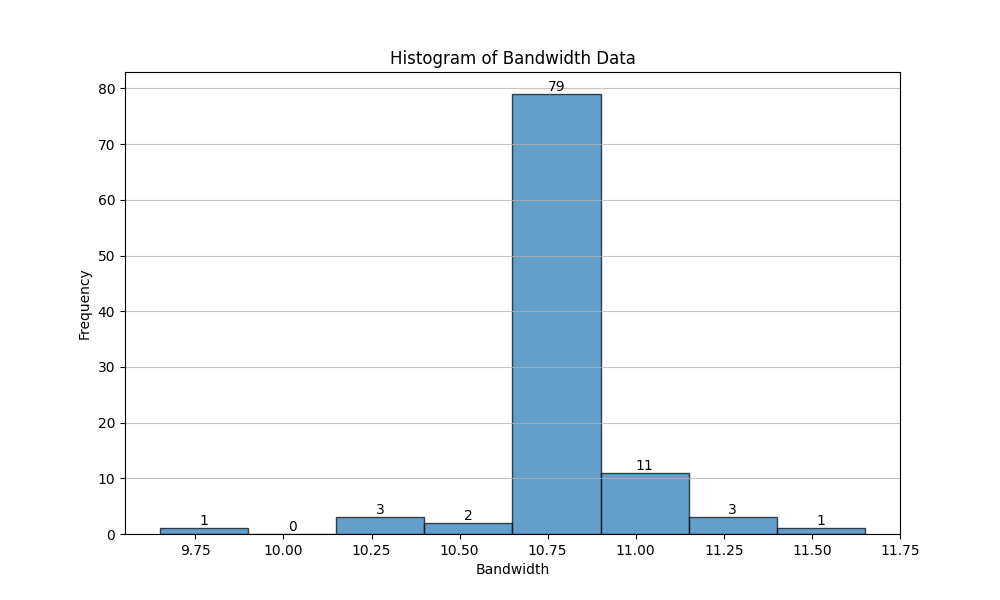
\includegraphics[width=0.8\textwidth]{bandwidth_histogram.png}
    \caption{Histogram of Bandwidth values}
\end{figure}


The bin size was set to be 0.25 Mbps. Yes, someone looking at the histogram can easily say that the bottleneck was set to be 10 Mbps because all the values are quite close to 10 Mbps. If we would have removed this protocol constraint, then histogram would have been spread out.


A peak of the histogram occurs around 10.75 Mbps (which is a little higher than the limit set by us). We have some values to the left and right of this peak too.





\end{solution}

\end{document}
